\section{Systems Architecture}

\subsection{System Overview Diagram}
% Content placeholder

\subsection{Electrical \& Power Systems}
% Content placeholder

\subsection{Electronic Control Units (ECUs)}
% Content placeholder

\subsection{Embedded Software Architecture}
\label{sec:embedded-sw-arch}

The embedded software running on the ESP32 microcontroller is structured as a \textbf{single-threaded, cooperative loop} built on the Arduino framework. This architecture was chosen for its simplicity and determinism: all BMS-related tasks execute sequentially on one core, eliminating the need for inter-task synchronization.

The software is divided into five logical layers, shown in Figure~\ref{fig:sw-layers}:

\begin{figure}[H]
    \centering
    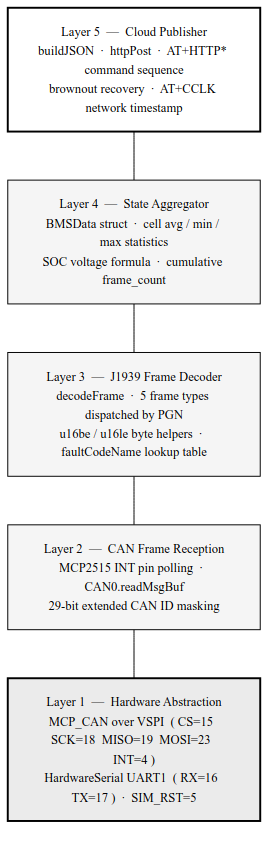
\includegraphics[width=0.25\textwidth]{images/sw-layers.png}
    \caption{ESP32 embedded software layer diagram}
    \label{fig:sw-layers}
\end{figure}

\begin{description}
    \item[Hardware Abstraction Layer (HAL)]
    Provides direct access to the MCP2515 via SPI (\texttt{mcp\_can} library) and to the SIM800L via HardwareSerial UART1. Pin assignments and bus parameters (CS, INT, baud rate, crystal frequency) are defined as constants and isolated from the application logic.

    \item[CAN Frame Reception]
    The MCP2515 asserts the \texttt{INT} line (GPIO 4) when a frame is placed in its receive buffer. The main loop polls this line and calls \texttt{CAN0.readMsgBuf()} to drain all pending frames. Extended CAN IDs are masked from the 29-bit field before processing.

    \item[J1939 Decoder]
    The \texttt{decodeFrame()} function dispatches each received frame by inspecting the \texttt{FUNC} byte of the CAN ID (bits 23--16). It handles five frame types (cell voltages, temperatures, BMS Basic 1 \& 2, charging request) and writes decoded values into the \texttt{BMSData} struct.

    \item[State Aggregator]
    The \texttt{BMSData} struct accumulates all decoded fields and maintains derived statistics (cell average, min, max, voltage-based SOC). The struct is updated in place and always holds the most recent complete state of the battery.

    \item[Cloud Publisher]
    Every 5 seconds, \texttt{buildJSON()} serializes \texttt{BMSData} into a JSON document using the ArduinoJson library, and \texttt{httpPost()} delivers it to the VPS via the SIM800L AT+HTTP* command set.
\end{description}

\subsubsection{Key Design Decisions}

\textbf{No RTOS.} A FreeRTOS task structure was considered but rejected because the single-responsibility loop handles all timing requirements naturally: CAN frames arrive at 100--500 ms intervals, and the publish cycle runs every 5 seconds. Adding preemptive scheduling would have introduced stack management and mutex overhead without any functional benefit.

\textbf{CAN drain during HTTP wait.} The SIM800L's \texttt{AT+HTTPACTION} response can take up to 30 seconds over slow GPRS. To prevent the MCP2515 receive buffer (6 frames deep) from overflowing during this window, the HTTP wait loop polls the CAN \texttt{INT} pin and drains frames continuously, calling \texttt{decodeFrame()} in-place. This ensures the \texttt{BMSData} struct is fully up-to-date when the next publish cycle begins.

\textbf{HardwareSerial over SoftwareSerial.} SoftwareSerial operates via bit-banging and is sensitive to interrupt latency. The SIM800L produces multi-line AT response bursts that SoftwareSerial occasionally drops bytes from at 9600 baud on a loaded core. HardwareSerial UART1 uses dedicated silicon and a hardware FIFO, making it robust under all operating conditions.

% ─────────────────────────────────────────────────────────────────────────────
\subsection{Cloud \& Connectivity Architecture}
\label{sec:cloud-arch}

The cloud and connectivity architecture connects the on-vehicle ESP32 to a remote browser with minimal intermediaries. The full pipeline is shown in Figure~\ref{fig:cloud-arch}.

\begin{figure}[H]
    \centering
    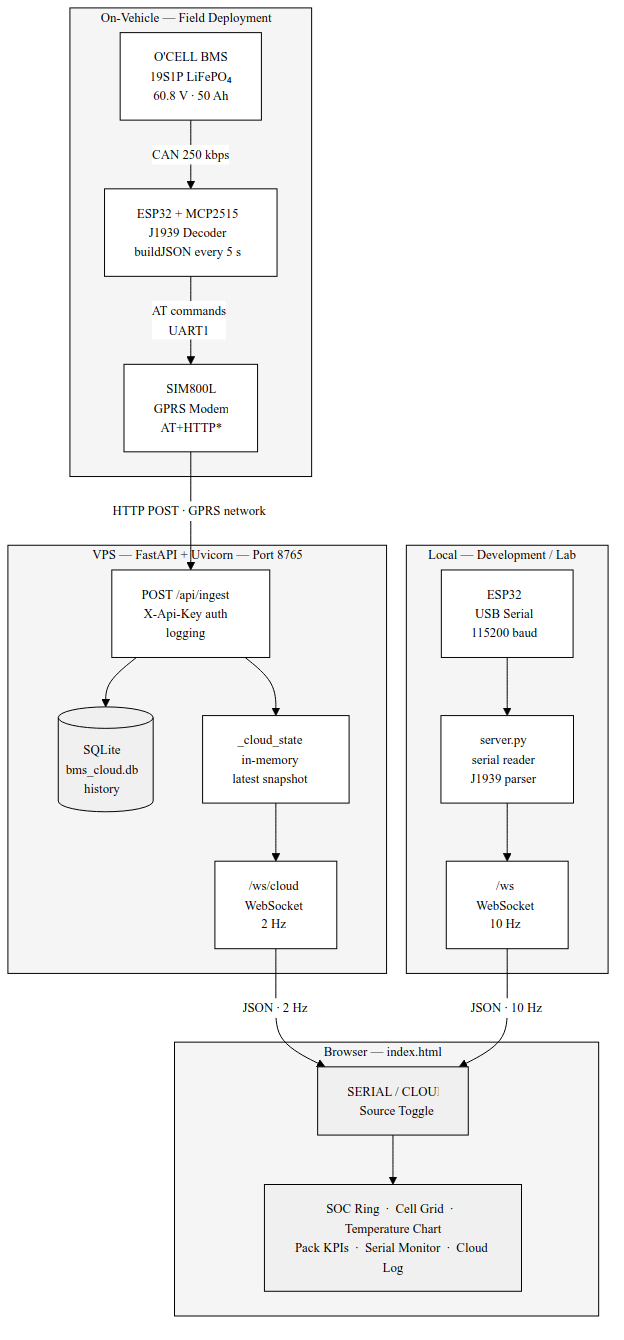
\includegraphics[width=0.5\textwidth]{images/cloud-arch.png}
    \caption{End-to-end cloud connectivity architecture}
    \label{fig:cloud-arch}
\end{figure}

\subsubsection{Component Roles}

\begin{description}
    \item[ESP32 + MCP2515 (On-vehicle edge node)]
    Reads and decodes SAE J1939 CAN frames from the BMS at up to 10 frames per second, aggregates them into a snapshot, and transmits one JSON document to the VPS every 5 seconds.

    \item[SIM800L GSM/GPRS Modem]
    Provides wide-area cellular connectivity using the carrier GPRS network. Communicates with the ESP32 via AT commands over UART. Handles TCP/IP, HTTP, and DNS entirely on-chip using the AT+HTTP* service, so the ESP32 only needs to manage the AT command dialogue.

    \item[VPS Backend (FastAPI + Uvicorn)]
    Acts as the single ingestion point and real-time relay for all cloud data. Receives POST requests from the ESP32, stores them to SQLite for persistence, and maintains an in-memory state that is pushed to connected browser clients via WebSocket at 2 Hz. The server also handles the SERIAL mode WebSocket, allowing the same dashboard to be used with a direct USB connection.

    \item[SQLite Database]
    Provides persistent local storage for all received snapshots. Enables historical data retrieval via the \texttt{/api/history} endpoint without any external database service.

    \item[Browser Dashboard]
    A single-page web application that renders live battery data received over WebSocket. Supports SERIAL mode (direct USB, 10 Hz) and CLOUD mode (VPS relay, 2 Hz). Auto-reconnects on network interruption.
\end{description}

\subsubsection{Data Flow Summary}

\begin{enumerate}
    \item O'CELL BMS $\rightarrow$ CAN bus (250 kbps, SAE J1939)
    \item ESP32 + MCP2515 $\rightarrow$ decode all frames $\rightarrow$ \texttt{BMSData} struct
    \item ESP32 $\rightarrow$ \texttt{buildJSON()} $\rightarrow$ JSON document
    \item ESP32 $\rightarrow$ SIM800L AT+HTTPACTION=1 $\rightarrow$ \texttt{POST /api/ingest} (HTTP, GPRS)
    \item VPS server $\rightarrow$ validate API key $\rightarrow$ SQLite insert + in-memory update
    \item VPS server $\rightarrow$ \texttt{/ws/cloud} WebSocket push every 2 s
    \item Browser $\rightarrow$ render panels (SOC, cells, temperatures, faults, cloud log)
\end{enumerate}

\subsubsection{Dual-Mode Operation}

A key architectural feature is that the dashboard supports two independent data sources via the same frontend interface. In \textbf{SERIAL mode}, the backend reads raw CAN log lines from the ESP32 USB serial port, decodes them through its own Python J1939 parser (\texttt{BMSState.decode()}), and pushes the result at 10 Hz. In \textbf{CLOUD mode}, the backend serves the latest snapshot received from the ESP32 over GPRS.

This dual-mode design provides two practical benefits:
\begin{itemize}
    \item During development and testing, the system can be operated entirely over USB without requiring a SIM card or GPRS connection.
    \item In the field, the dashboard can be opened from any web browser pointed at the VPS IP address, with no local software to install.
\end{itemize}

\subsection{3D Mechanical Architecture}
% Content placeholder

\subsection{Safety \& Redundancy Design}
% Content placeholder
